\documentclass[12pt,twoside]{report}
\usepackage[utf8]{inputenc}
\usepackage{graphicx}
\usepackage{authblk}
\usepackage{hyperref}
\usepackage[backend=biber]{biblatex}
\addbibresource{res.bib}
\usepackage[a4paper,width=150mm,top=25mm,bottom=25mm]{geometry}
\usepackage{fancyhdr}
\pagestyle{fancy}
\fancyhead[RO, LE] {\title}
\fancyfoot{} % clear all footer fields
\fancyfoot[LE,RO]{\thepage}
\fancyfoot[LO,CE]{Mohsen Dehbag}
\fancyfoot[CO,RE]{Chapter \thechapter}

\usepackage{xcolor}
\usepackage{listings}
\definecolor{mygray}{rgb}{0.8,0.8,0.8}
\lstset{%
basicstyle=\ttfamily,
breaklines = true,
backgroundcolor=\color{mygray},
}
\usepackage{realboxes}


\usepackage{amsmath}
\usepackage{booktabs}

\graphicspath{{images/}}
%
\newcommand*{\email}[1]{%
    \normalsize\href{mailto:#1}{#1}\par
    }

\title{
{Creating a cryptoCurrency with blockChain Technology}\\
{\large Technical and Vocational University (Shahid Shamsipour)}\\
{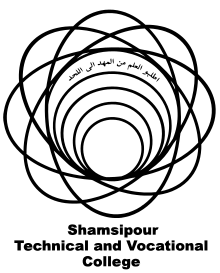
\includegraphics[width=150px]{image/shamsi.png}}
}
\author{Mohsen Dehbag\\ \email{mohsendehbag@icloud.com}}
\date{March 2020}

\begin{document}

\maketitle


\chapter*{Abstract}

Blockchain  has been the Most influential  technology since the past decade. The firs word that comes to mind after writing about blockchain is bitcoin, although many people still confuse the blockchain technology with the bitcoin it self however, bitcoin and cryptocurrency are just one of the applications  of blockchain.  In addition to decentralizing money and payments, the system can also be sent to other participants on the network for registration, approval and sending of contracts. This technology in our country can bring about major changes due to the pressure of foreign governments, including the possibility of transferring currency to all other countries without the need for sanctions, and it can be used to accelerate, increase security and transparency of transactions within the country. Also used.
To further introduce Blockchain, it is a decentralized, digital office and database that is used for the secure exchange of information, digital currency, transactions, and transactions. Each member of the network has access to the latest encrypted Office version so that they can approve or send a new transaction. Basically this is a distributed database that holds and grows a block. Completed blocks are added in chronological order. Each block contains a timestamp and the information link pointing to the previous block.\\
\textbf{Keywords:} Blockchain-Cryptocurrency-Bitcoin

\chapter*{Dedication}
To Mom and Dad who supported me everyday and moment and myself.

\chapter*{Acknowledgements}
I want to thank Amir Hossein Aghaie and Ali Reza Rabeyi for their Tremendous amount of help through finishing this project.


\newpage
\Large Created with \LaTeX{}
\tableofcontents

\chapter{Introduction}
\input{chapters/cahpter1}

\chapter{A review of related work}
\section{Preface}
There have been various projects with different goals since the first crypto currency or bitcoin was built. The purpose of using this technology is to enhance transparency, security and speed and is commonly used in services where these three factors are particularly important.
Bitcoin, for example, uses all three factors. Apps like Spotify and Steam have used its transparency feature in their apps. And programs like Storeke have borrowed security from this technology.
\section{Examples of smart contract applications in Blockchain}
This Technology is being used by so many branches and it speeds off the functionality of the organizations that its being used in in this section we analyze some of those sections.

\subsection{In medical}
The technology has also been used in various fields and disciplines; personal health records can be encrypted and stored with a private key and accessed only by specific individuals. The same strategy can be used to ensure that investigations are conducted through HIPAA rules (in a secure and confidential way). Surgical receipt can be kept in chains and sent automatically to insurers as proof of delivery. It can also be used to manage public health care such as medication monitoring, compliance, test results, and management of health care resources.
\subsection{In Music Industry}

The 2017 Hype Cycle report (Gartner Inc. 2017) suggests that the technology is five to 10 years away
to mainstream adoption. The report expects that during these time, some focus will be given to create
convergence in architectural styles (private and public) resulting in all distributed ledgers having
similar functional characteristics. Moreover, it is also states that “concerns remain about the viability
of the technologies, security (software and hardware), scalability, legality and interoperability”,
especially given that public ledgers seem inappropriate for most enterprises internal information.
However, even with the technology in its initial stages of development, for the purposes of
disintermediation in the music industry, it shows great immediate potential. Two of the main issues
identified in our research are:
1. the lack of access to transactional information; and
2. the inefficiencies associated to royalty payments;
Blockchain technology can solve both of these issues, while maintaining transparency
throughout the entire chain. Not only that, as we will discuss in section 5, the possibilities for
applications go beyond the traditional business models in the industry, enabling a closer relationship
between Artists and Consumers. 
For the music industry specifically, the addition of blockchain powered models may result in a
complete change of the industry’s structure. Some of the main issues identified by the analysis of its
supply chain models were the lack of transparency through the chain, musician’s low bargaining
power, and inefficiency of the royalty payments systems. Through the use of applications such as
record keeping, smart contracts and metadata analysis, these issues may be eliminated and
intermediation turned obsolete.
It is important to note, however, that even with all the potential benefits to the music industry, the
new business models introduced with the technology are also in their initial stages. The mere fact that
they function through the use of cryptocurrencies, not money, may still be too controversial to some consumers. Due to the novelty of blockchain and the platforms powered by the network, the ability
to project the success of these models is quite limited.
Another point worth mention is the fact that without a revenue stream, it is unclear how these music
platforms will continue to develop and reach consumers with the same power as their competitors
Spotify and Apple Music. All three analysed platforms (Musicoin, Resonate and Ujo) have mainly
independent artists and labels in their catalogues, making it unlikely a scenario in which those artists
would have the means to finance the projects. At the same time, by charging for the use of the
platforms, there would be no disintermediation, only an exchange of it. With time, it is possible that
the value captured by the artists would go back to decrease and intermediation power to increase.
Nevertheless, it is undeniable that blockchain technology can bring innovative business models to
the music industry. The expectation is that new enterprises start to develop applications using the
technology and increasing the total amount of usage for corporations and consumers. Furthermore,
the involvement of mainstream and independent artists in this process may be of great contribution
for the dissemination of blockchain in the music industry.
Due to the initial stages of development, it was difficult to access enough data regarding the
performance of the platforms already in use. Ideally, comparing the results of those blockchain
powered platforms with the initial results of their competitors using the subscription model could
indicate how far they are from mainstream consumption. Similarly, not a lot of research was applied
to blockchain in the music industry. Not only literature is limited, but also the perception of the
effectiveness of the technology to this industry in particular.
From this research, we have the intention of further evaluate the phase of development of
blockchain in the music industry by analysing it from a performance and adoption, by artists and
consumers, perspective.\textcite{sitonio2018impact}

\subsection{In governmental processes}
In the 2016 US election, Democrats and Republicans questioned the security of the voting system. The Green Party demanded recounts in Wisconsin, Pennsylvania and Michigan. Computer scientists say hackers can cheat by manipulating the electronic system as a result. The manual prevents fraud during encryption. Private individuals can confirm that their votes have been counted and confirm who they voted for. This system saves only the government.
According to a 2013 report from McKinsey and Company, open data - open source government data available to all citizens through the Internet - provides a platform for fraudsters to use its data to fraud, allowing farmers to track time. Carefully harvest the crop in the field, and parents can research the side effects of the drug for their sick children. Currently, this data is only published once a year and is largely unaccountable for citizen input. As a public notebook, the block chain system can open this data to citizens whenever and wherever it wants.

\section{Examples of block chain powered} government applications
Block Chain technology can be used for any transaction or information exchange that takes place in which the government is involved. The fundamental characteristics of this technology enables implementation in a wide range of processes for asset registry, inventory, and information exchange, both hard assets like physical property, and intangible assets like votes, patents, ideas, reputation, intention, health data, information etc. (Swan, 2015). The essence of a BC is that organizations can keep track of a ‘ledger’ and that organizations jointly create, evolve and keep track of one immutable history of transactions and determine successive events.
Governments from all over the world are conducting pilots using BCT. Government BC applications are diverse in nature and include digital identity, the storing of judicial decisions, financing of school buildings and tracing money, marital status, e-voting, business licenses, passports, criminal records and even tax records (see for examples Blockchain Projects, 2017). We recommend further research to compare the variety of initiatives and to analyze the source of benefits.
The BC technology requires situations in which multiple parties are involved in a transaction. A notable example is granting permits to the organizers of mass events, like concerts and demonstrations, which requires the municipality, police, fire brigade and health organizations to agree and to ensure they are prepared for dealing with the mass. Another example is the transfer of car ownership. To find a car owner, the car's transaction history has to be analyzed assuming that it contains an unambiguous property identifier. The owner of the car can be identified by searching a ledger as everybody has the same view on the BC. The rule states that only the owner can sell the car. When the car is sold a transaction needs to be created in which the previous owner confirms selling the car, the new owner confirms buying the car and the bank (or another party) confirms the payment for the transfer of the ownership. Another example is keeping an overview of the authorities provided in a public organization and the ability to change the authority only if there is agreement among nodes which are classified as being higher ranked in the hierarchy. As such, BC is a technology that replaces single databases by a distributed ledger of shared information, which should result in higher security and accessibility. This difference is schematically depicted in Fig. 1. Each node in the network contains a full copy of the BC, the transactions are recorded in the ledger and each node has access to the full history of transactions. Access to the ledger can be restricted, and the number of nodes as well as the type of consensus mechanism need to be determined. These choices influence the stewardship role of government, which we address in more detail in Subsection 6.5.
A final example is the use of BCT for land title projects. This BC applications is particularly useful when ownership records are not preserved in a systematic way or the operating organization is not trusted. In some countries the ownership of a land title is hard to detect. By using a BC application every transaction of land property should be registered. BCT prevents manipulation and loss of data. The transfer of land property requires that the lawful owner has to sign, for which there should be proof of ownership, no left mortgage should rest on the land property, and a payment (money transfer) from the buying to the selling party has to be made. BC can be used to protect the rights of the owner of the land, to resolve disputes, to make sure that ownership is correctly transferred and to prevent any unauthorized and fraudulent changes. However, BCT does not help to address the accuracy of the land titles, but rather seeks to clarify the authenticity of the title. In the case that input is manipulated and still complies with the conditions it will nevertheless be accepted by the network and added to the BC. Hence BC can be used as one of the instruments to fight corruption with land registries, but should be part of a wider institutional setting including other instruments for a legally correct and compliant land registry administration.
These examples show that BC applications can have significant effects on the way organizational processes are designed. E.g. in the case of using a BC applications for land registry organizations involved in land registry processes can directly interact with each other. This reduces the mediating role of the land register organizations who only need to focus on developing, maintaining and governing the BC application. Yet, if and how such organizations should be transformed to serve as owners and guardians of the BC application is still an open question. To the best of our knowledge, there are no deep analyses of these changing administrative processes and organizations in their institutional context yet and research in this area is required.
Some authors even go one step further by arguing that BC is “an institutional technology of governance that competes with other economic institutions of capitalism, namely firms, markets, networks, and even governments” (Davidson, De Filippi, and Potts, 2016, p.1). Atzori (2015) even stated that BC can be viewed as technology that competes with the role of government in society. Technology competing with an institution might be considered as a technology-push, far-fetched and naive, but nevertheless such propositions should not be ignored and research is needed to position this in a more realistic view which takes into account both technical and institutional elements. What the BCT has to offer is that instead of transactions being handled directly by government organizations, they can be handled by distributed ledger technology running on P2P platforms that are enabled and facilitated by (or on behalf of) government organizations. This raises questions about who will set-up, execute and maintain these architectures which will likely still be the role of government, but the actual transactions might be performed without the government.\textcite{olnes2017blockchain}

\subsection{Public and community value}
The collection can facilitate self-organization by providing a self-management platform for companies, NGOs, foundations, government agencies, academics and individual citizens. Parties can interact and share information globally and transparently - think of iCloud and google drive, but it's bigger and less risky.

\subsection{Assignment of responsibility}

By using blockchain, the use of responsibilities is clearly and transparently communicated to those responsible, such as students, administrators, staff, and department heads.
This will identify all work done at the academic, team and community level and encourage fine-tuned individuals and people who are doing their job properly.

\subsection{Identity in cyberspace}
Whether we like it or not, online companies know everything about us. Some of the companies we buy online sell their identity information to advertisers who send you their ads. By creating a protected data point, Blockchain allows you to be safe from these abuses and to show everyone who needs your information only that particular area.

\subsection{Passports}
While there exists somewhat imperfect systems for establishing personal identity in the real
world, in the form of identity document, driver’s licenses and even passports, there is no
equivalent system for securing either online authentication of our personal identities or the
identity of digital entities. So while governments can issue forms of physical identification, online
identities and digital entities do not recognize national boundaries and digital identity
authentication appears at first look to be an intractable problem without an overseeing global
entity.
Blockchain technology may offer a way to circumvent this problem by delivering a secure
solution without the need for a trusted, central authority. It can be used for creating an identity on
the blockchain, making it easier to manage for individuals, giving them greater control over who
has their personal information and how they access it.
By combining the decentralized blockchain principle with identity verification, a digital ID can be
created that would act as a digital watermark which can be assigned to every online transaction.
The solution can help the organizations to check the identity on every transaction in real time,
hence, eliminating rate of fraud. Consumers will be able to login and verify payments without
having to enter any of the traditional username and password information. Through blockchain
solutions, consumers can simply use an app for authentication instead of using traditional
methods, such as a username and password. The solution will store their encrypted identity,
allowing them to share their data with companies and manage it on their own terms.\textcite{jacobovitz2016blockchain}

The first digital passport was launched in 2014 on GitHub and can help owners identify themselves online and even offline abroad. how it works? You take a picture of yourself, stamping it with a public and private key, both of which are encrypted to prove it. According to the Bitcoin address, the passport is stored in a general IP in the booklet and is verified by the users of the blockchain.
In general, this application of blockchain includes the creation of death, birth, marriage and birth certificates. It also retains its functionality for all ID cards.

\subsection{Energy supply}
In some parts of the world, businesses and homes can take advantage of blockchain-based distribution networks to store energy and accurately track consumption. Blockchain can also be used to improve the pursuit of clean energy. When electricity is sent to the grid, no one can tell if it was produced by fossil fuels or wind or solar energy.
Traditionally, renewable energy is tracked by government-approved transferable licenses. These permissions have problems that "blockchain" can solve.

\subsection{Accounting}
Transaction recording through blockchain significantly eliminates human error and saves data from possible tampering. Remember that records are approved each time a new block is generated. Of course, the whole accounting process is also more effective. Instead of keeping separate records, businesses can keep only one general ledger. The integrity of a company's financial information will also be guaranteed.

\subsection{Stock market}
The concept of using blockchain technology for security and exchange of goods has been around for some time. Due to the open and secure nature of the blockchain system, the stock market is also looking at blockchain technology as a jump point. The Australian stock market has long been planning to move its operations to a blockchain-based system, designed by the startup blockchain Digital Asset Holding.

\subsection{Internet of things}
The combination of these two technologies increases their speed and ease.

\section{Conclusion}
It is important to note that working with Black China, if these standards are met, can become a powerful tool for doing and improving business, making the global economy fairer, and helping to support more open and fair societies.
Now, with the application of this technology and the tools made with its help, it is possible to write a complete program example for the vulnerable points of the society. Blockchain is an emerging technology that requires compatible applications. A set of rules must also be set for the use of this technology. This technology must be able to prove its effectiveness in order to be widely used.



\chapter{Development environment configuration method}

\section{Introduction}
In the beginning of section, we will look at the environments in which this program was developed, then we will introduce the concepts and configurations in this system, the blockchain.

\section{Programs and services used in project construction}
For the creation of the project we need to have access to several technologies we 

\subsection{Visual studio code}
Visual Studio Code (or VSCode for short) is one of the most popular code editors created and maintained by Microsoft. VSCode supports a wide range of programming languages, including languages such as Python, PHP, JavaScript, HTML, CSS, ASP.NET, Java, and many other languages. The second and perhaps most important point is that it's free, because it doesn't have the problems of breaking the lock and legal issues, but the obvious feature that makes it even more brilliant is the support for plugins.\textcite{wiki:Visual_Studio_Code}

The different parts of this program are:

\begin{itemize}
\item Explorer:
\end{itemize}

This is the structure of your folders and files. Clicking Explorer will open a menu that displays all the files and folders of the current project, and you can create new files or folders using the small icons at the top.

\begin{itemize}
\item Search section:
\end{itemize}

This section allows you to search for a specific section of code or replace specific code with other code.

\begin{itemize}
\item Source Control Management:
\end{itemize}
This section is for version control systems such as Git. Systems like Git help you better manage your project source code and prevent unwanted code deletion. They are also an ideal choice for group work on a project.

\begin{itemize}
\item Debugging section: 
\end{itemize}
As its name implies, it is responsible for debugging. Note that depending on the language of your program, you may need plugins to debugging.

\begin{itemize}
\item Extensions section: 
\end{itemize}
This section allows you to search for different plugins and add them to VSCode. These plugins are designed for a variety of purposes, for example: visual beauty and themes, support for frameworks such as React or Vue, increased support for some programming languages such as Python, improved quality of certain parts of VSCode such as debugging, and more.

\subsection{Post Man}
Postman is an API testing is a type of software testing that involves testing application programming interfaces (APIs) directly and as part of integration testing to determine if they meet expectations for functionality, reliability, performance, and security. Since APIs lack a GUI, API testing is performed at the message layer. API testing is now considered critical for automating testing because APIs now serve as the primary interface to application logic and because GUI tests are difficult to maintain with the short release cycles and frequent changes commonly used with Agile software development and DevOps.\textcite{wiki:API_testing}

One of the reasons for using my post is that it is free, easy to share, and get code output for each of the APIs, which means that anything that can reduce programming and development time is very important. One of these features is Code Snippet, which allows you to have an output in your favorite programming language after scheduling and testing each API. Languages such as JAVA, Csharp, PHP, Python. Also, its multi-platform makes it possible to run and edit on all devices.

\subsection{Python Language}
Python is an interpreted, high-level, general-purpose programming language. Created by Guido van Rossum and first released in 1991. Python's design philosophy emphasizes code readability with its notable use of significant whitespace. Its language constructs and object-oriented approach aim to help programmers write clear, logical code for small and large-scale projects.

Python is dynamically typed and garbage-collected. It supports multiple programming paradigms, including structured (particularly, procedural), object-oriented, and functional programming. Python is often described as a "batteries included" language due to its comprehensive standard library.

Python was conceived in the late 1980s as a successor to the ABC language. Python 2.0, released in 2000, introduced features like list comprehensions and a garbage collection system capable of collecting reference cycles. Python 3.0, released in 2008, was a major revision of the language that is not completely backward-compatible, and much Python 2 code does not run unmodified on Python 3.

The Python 2 language, i.e. Python 2.7.x, was officially discontinued on 1 January 2020 (first planned for 2015) after which security patches and other improvements will not be released for it.With Python 2's end-of-life, only Python 3.5.x and later are supported.

Python interpreters are available for many operating systems. A global community of programmers develops and maintains CPython, an open source reference implementation. A non-profit organization, the Python Software Foundation, manages and directs resources for Python and CPython development.\textcite{python}

The latest version of Python 3.5 was introduced at the time of its development, but due to the support of the Python team, Python 3.8 was also available for use when writing this article.
Due to the many problems that exist on the Windows operating system, to work with the server and for the Python programming program, after designing the basic parts of this program, it continued to develop with Linux, Arch, but due to the complexity of installing it in this article. The installation of Python on the Linux Ubuntu operating system is described.
Installing Python using the pacman tool is a very simple process. The following steps are required to install Python on Linux (arch distribution) by the pacman tool.
\linebreak

% demo using \lstinline and \Colorbox
\Colorbox{mygray}{\lstinline|sudo pacman|}
\linebreak

Once the PPA software has been activated, install version three of Python using the following command line:
\newline

\Colorbox{mygray}{\lstinline|pacman -S python|}
\linebreak

in the end by typing python3 in terminal you can see if the installation was successful or not.

\subsection{Virtual environments}
One of the most important methods tested is Python. Whenever you want to start a new Python project, you need to decide which version of Python you want to use. You will also need to choose from some libraries or packages. Of course, another way is not to install these packages on a system level. Because it's possible to always work on different projects that require different versions of Python. At the same time, you may need some special packages that only work with one version of Python and work on other versions. In such cases, we need to create different environments for Python. These environments are called Python Virtual Environments. The virtual environment used in this program will vary depending on what system and how you install Python on the system. However, if you've installed Python 3 using Homebrew, its location on the system will be as follows:

\Colorbox{mygray}{\lstinline|/usr/local/Cellar/python/3.7.2_1/bin|}


In this case, you can use the following command to install virtualenv using pip3:


\Colorbox{mygray}{\lstinline|pip3 install virtualenv|}


Now all the packages are installed and we can start setting up the virtual environment. We must first determine where we want to build our environment and name it. We create our virtual environment in the same directory where we installed it, and name it virtEnv1:

\Colorbox{mygray}{\lstinline|virtualenv -p python3 ~/virtEnv1|}

To enter and activate a virtual environment called my env, we do the following in windows:

\Colorbox{mygray}{\lstinline| cd Documents\SampleENV\Scripts\ , activate.bat|}

and in Linux and macOS venv can be activated by:

\Colorbox{mygray}{\lstinline|cd Documents/SampleENV/ , source bin/activate|}

\textbf{Advantages of Virtualenv:}

It can be easily upgraded using pip and can easily work with different versions of Python. It also supports Python 2.7 and later.

\textbf{Disadvantages of Virtualenv:}

In this virtual environment, the interpreter's binary file is practically copied to a new location and must be read from there. Also, if you want to use it, you have to install it separately and it will not be provided with Python.
Notice how the prompt of the command line changes as you successfully enter the virtual environment.
We can now access libraries, pip, site-packages directory, and proprietary commentary in our project. Also, by activating a virtual environment, the executable files related to this environment are placed inside the PATH variable so that they can be easily accessed as if the commands were used.
In Linux, you can check which python3 and which pip3 to execute by executing commands.
So, for each project, it is enough to create a virtual environment within the project once by calling virtualenv, and then activate that environment every time you enter the project directory.
To exit and deactivate the environment, use the following command:

\Colorbox{mygray}{\lstinline|(SampleENV) deactivate|}

\subsection{vue.js}
Vue.js is an open-source Model–view–viewmodel JavaScript framework for building user interfaces and single-page applications.
It was created by Evan You, and is maintained by him and the rest of the active core team members coming from various companies such as Netlif and Netguru.\textcite{wiki:Vue.js}
To install Vivo, you must first install node.js. To do this, you must first install the desired package from the site https://nodejs.org/en/. You can use the following command to install the latest version of Vue CLI: \newline

\Colorbox{mygray}{\lstinline|npm install -g @vue/cli|}\newline

\subsection{Axios}
Promise based HTTP client for the browser and node.js\textcite{axios}

with this frameWork we can
\begin{itemize}
\item Make XMLHttpRequests from the browser
\item Make http requests from node.js
\item Supports the Promise API
\item Intercept request and response
\item Transform request and response data
\item Cancel requests
\item Automatic transforms for JSON data
\item Client side support for protecting against XSRF
\end{itemize}

Axios should be installed from YAM repository:

\Colorbox{mygray}{\lstinline|npm install axios --save|}\newline

\subsection{Peer to Peer Network}
Similar to P2P refers to a specific type of computer network that uses a distributed architecture. This means that all computers or devices that are members of this network share their workload on the network. Computers or devices that are part of a unique network are called peers. Computers within a unique network have no preference over each other and are all equal. Computers within a unique network share resources between each other without the need for a centralized management system.
Similar networks, while being used to share resources, also help computers and devices provide a specific service in the form of a group or perform a specific task. However, the above networks are mainly used to share files on the Internet. P2P networks are ideal because they allow computers to connect to the network and simultaneously process and receive files. Suppose you open your browser and open a website to download a file. In this case, the site works as a server and your computer receives a file as a client. This is similar to a one-way street. The file you are downloading is a machine that moves from point A (site) to point B (your computer).
If you download the same file through a similar network, for example through a torrent site as a starting point, the download will be done in different ways. The file is downloaded in the form of bits and sections that are on different computers within a similar network. At the same time, a file may be sent from your computer to the computers that requested the file. This situation is similar to a two-way road.
Advantages and disadvantages of P2P
We now turn to the strengths and weaknesses of this architecture.

\textbf{Advantages}:

The peer-to-peer structure provides many benefits. Among the most important advantages of P2P, it can be said that peer-to-peer networks provide much more security than traditional customer-server settings. The distribution of blockchains in a large number of nodes makes them immune to Dos, which affects countless systems.
Similarly, since a large number of nodes must reach a consensus before data can be added to the blockchain, it is almost impossible for an attacker to change the data. This is especially true for large networks such as Bitcoin. Smaller blocks are more prone to attacks, as one person or group may eventually be able to take control of the majority of nodes (this is known as a 51 percent attack).
As a result, the peer-to-peer distribution network, coupled with the need for a consensus of the majority, gives the "blockchain" a great deal of resistance to malicious activity. The P2P model is one of the main reasons why bitcoin (and other "blockchains") is able to withstand the Byzantine error.
In addition to security, the peer-to-peer structure of cryptocurrencies can make them resistant to censorship by central authorities. Unlike standard bank accounts, cryptocurrency wallets cannot be blocked or emptied by governments. This resistance is also created by the efforts of content platforms and the processing of private payments for censorship.
Some content producers and online traders have chosen to use cryptocurrencies as a way to prevent third parties from blocking their payments. After stating the advantages of P2P, we go to its disadvantages.\pagebreak

\textbf{Disadvantages}:

Despite the many benefits and advantages of P2P, like any other concept, it has its drawbacks and limitations.
Since the general offices have been redesigned, instead of a central server, they must be updated in all ninety, adding a transaction to blockchain requires enormous processing power. Although this provides a lot of security, it greatly reduces efficiency, and is one of the main barriers to scalability and widespread acceptance.
However, cryptocurrency developers and developers are looking for alternatives that can be used as a scalability solution. Highlights include the Lightning Network, Plasma Atrium, and the Mimbel Wimble protocol.
Another limitation of peer-to-peer networking could be related to the attacks that took place at hardfork events. Since most blockchains are decentralized and open source, groups of ninety can freely copy and modify code, break away from the main chain, and create a new parallel network. Hard forks are completely normal in themselves, and there are no threats. However, if certain security issues are not properly addressed, both chains may be at risk of attack.
In addition, the distributed nature of P2P networks makes them relatively difficult to control and regulate. Several programs and companies have been involved in illegal activities and copyright infringement.

\subsection{CLI Programs}

A command-line interface (CLI) processes commands to a computer program in the form of lines of text. The program which handles the interface is called a command-line interpreter or command-line processor. Operating systems implement a command-line interface in a shell for interactive access to operating system functions or services. Such access was primarily provided to users by computer terminals starting in the mid-1960s, and continued to be used throughout the 1970s and 1980s on VAX/VMS, Unix systems and personal computer systems including DOS, CP/M and Apple DOS.

In computer system configuration, CLI is still widely used. These days, CLI is mostly done by software programmers or system administrators to perform some of their important tasks, otherwise it will take a lot of time and effort if the GUI is running.
For this project, a node is created with a graphical user interface (GUI) and a command user interface.

\section{Conclusion}
By using the architectures and technologies mentioned above we get one step closer to completing the program.


\chapter{Analysis and design}
\section{Preface}
As discussed in previous articles, emerging blockchain technology is based on a series of rules and frameworks that try to look at what's going on inside the blocks and the process of building a block.
If a person sends a request on the network, the request will be verified by the network service providers or so-called nodes, then the request will be placed in the form of a transaction within a block.

\section{Definitions}

To begin to understand cryptocurrency, we have to examine the technology that powers it, and consequently, certain concepts to which cryptocurrency owes its existence. Let us first start by defining what cryptocurrency is. 


\subsection{Basic Definitions}

\begin{table}\centering
    \renewcommand{\arraystretch}{2.5}

    \begin{tabular}{@{}c|l@{}}
            \bfseries Phrase & implication\\
            \hline\hline
            Miner
            & 
            Transaction confirmer\\
            Public agreement
            &
            A V based method for accepting the transaction.
            \\
            Forking 
            & a fork is what happens when a blockchain diverges into two potential paths forward — 
            \\
             
            &
            either with regard to a network's transaction history or a new rule in deciding what makes 
            \\
            
            &
            a transaction valid. But forks also can be willingly introduced to the network.
            \\
            hash 
            &
            Applying hash is a way to check the accuracy of a transaction
            \\
            Node
            &
            A ledger in user side of block Chain.
            \\
            Time Stamp
            &
            Variables or variables to record time spent on blockchain
    \end{tabular}
\end{table}
\pagebreak

Table number one. An overview of widely used concepts 
\textcite{tasatanattakool2018blockchain}
\linebreak

\raggedright\subsection{General Definitions}
Blockchain:
A chain of blocks that each block contains valuable data without monitoring from the central server. This information is protected by encryption and cannot be changed.
Decentralized Blockchain:
Blockchain has a decentralized structure due to the lack of a central server.
Public Consensus:
Before new information is added to Blockchain, more than half of ninety people must confirm that this new information is valid for Blockchain.
Unchanging:
Once the information is added to the blockchain, it cannot be changed or deleted. The information is protected by blockchain, so the information is encrypted and makes it almost impossible to hack the information.
Extractor:
Users who use their computer power to extract blocks.

\section{Processes of Creating a blockchain }
Ethereum developer Vlad Zamfir says that cryptoeconomics is “A formal discipline that studies protocols that govern the production, distribution, and consumption of goods and services in a decentralized digital economy. Cryptoeconomics is a practical science that focuses on the design and characterization of these protocols.” The blockchain technology runs on the principles of cryptoeconomics as implied by the word Cryptoeconomics coming from the combination of Cryptography and Economics. The cryptoeconomy consists of cryptoeconomic approaches by combining cryptography and economics to create robust and decentralized Peer-to-Peer networks that thrive over time despite adversaries that attempt to disrupt the network. The cryptography underlying these systems is what makes the Peer-to- Peer communications within the networks secure and the economics are what incentivizes all actors to contribute to the network so that it thrives over time and to be applicable to traditional economic activities as well as newly created ones in terms of users, distributed capital markets, applications, services, micro payments, live collaboration, and auctions.\textcite{choecreating}
\subsection{Process 1: Create an address}

You need to have an address to connect to the ChinaBlock network. Creating an address is not difficult and time consuming, but it is necessary to connect to the network. Your URL consists of two parts, a public URL and a private URL, in which the URL is a URL that must be available to you and is your signature. Anyone with easy access to your private URL can do anything. Count on you, including stealing digital assets in that node.

\subsection{Process 2: Encryption}
Your request will be sent to the network with your signature (which is done via a private key) and this request will be verified through your public key, whether the request is digital currency transfer or just sending a text.
Whatever you want to do, it will be encrypted! If you want to send, for example, "Hello Sepehr" to someone, the word is encrypted through the hash pan and becomes a series of letters and meaningless numbers in the door. For example, "Hello Mohsen" becomes "bce9c72c24edbd3baa1d3cac4d457d45".
\newline

\centering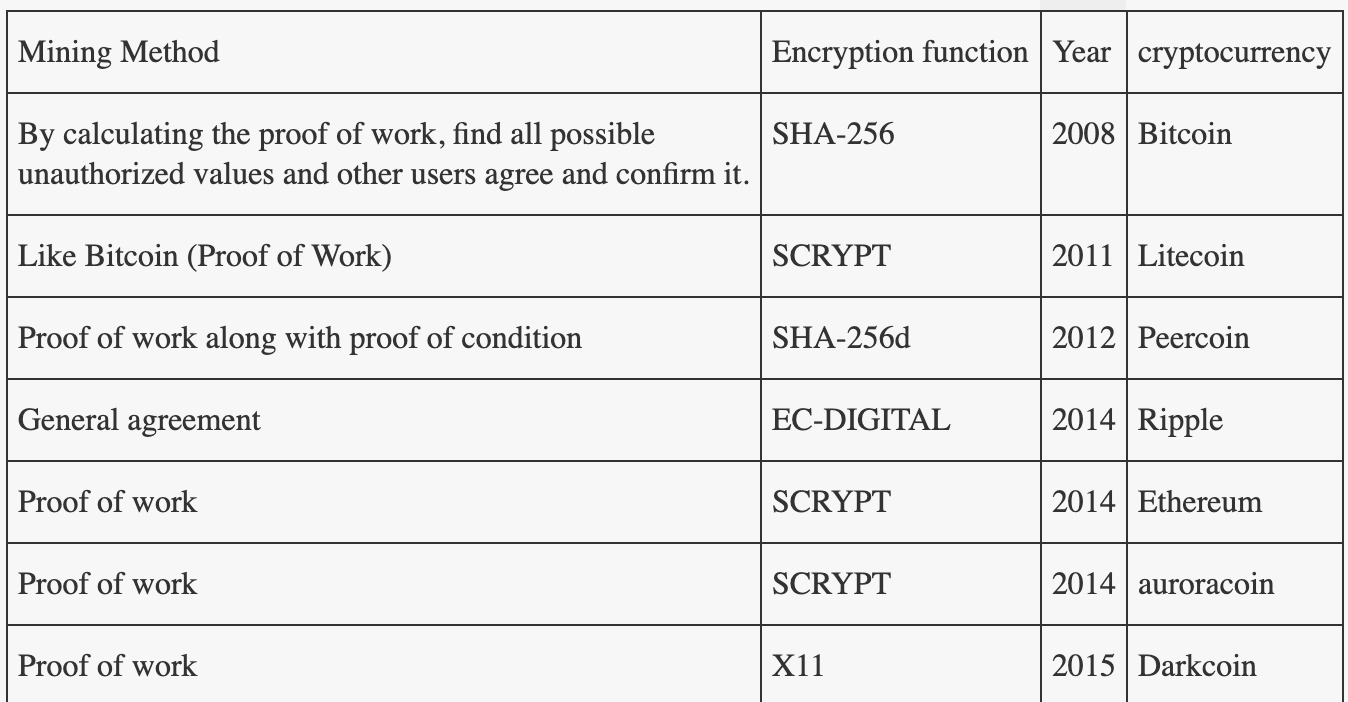
\includegraphics[width=15cm, height=7cm]{image/table2.png}
Table Two. General information about currency codes\textcite{tama2017critical}
\pagebreak
\begin{flushleft}
\subsection{Process 3: Prevent recurrent hashes}

The question may be, what if the same data is available? In the same way that the same hashes are created!
For example, consider a transaction with the same data being sent from one address to another, in which case duplicate hashes are generated, because everything is the same. The network has come up with a solution to this problem.
\section{Nonce}

Nans is made for this purpose, Nans is a random value that is added to the data and is created after the addition of a new hash, in which case the same data will not have the same hashes.
Process 5: Blockchain formation
In blockchain, each block depends on its previous block, so that when a series of transactions are placed in a block and in general that block is hash, this hash (which contains information from all previous transactions) is placed in the next block. Until the end…
• First of all, this is why they say the blockchain chain, because in each hash block there is a previous block and the chains are connected together.
• Secondly, this is why changing the information in each block causes the connection between the blocks to be disrupted, because even if the hash of a data change, the hash of all blocks changes.
This is not hidden from network members, so if someone wants to make a change, the network service providers will notice the change and will not approve it, unless 51 percent of the service providers accept the change and accept it.
According to the mentioned concepts, the level of security and transparency can be observed in the structure of "blockchain" and the way this network works can be interesting for those who are interested in its type.

\section{Data structure}

Deep and practical knowledge of data structure is essential when the goal is to become a blockchain developer. Blockchain developers are constantly displaying and optimizing existing data structures such as the Merkel Tree, the Petersia Tree, etc. to meet the needs of their personal network. Blockchain uses many data structures to build a secure and unchangeable system using advanced encryption. Knowledge of blockchain is incomplete without sufficient information about the structure of the data.

\section{Cryptography or encryption algorithm}

As mentioned earlier, blockchain is a combination of data structure and advanced encryption. Thus, it is clear that a good understanding of cryptography is essential for a blockchain developer. Many encryption methods, such as hash functions, such as SHA256 and KECCAK256, are used to generate digital signatures on blockchain instead of asymmetric encryption. Without an understanding of how they work, it becomes virtually impossible to develop a blockchain developer.

\section{Web Development}

Web development is a key aspect of blockchain development. When a person starts out as a blockchain developer in the industry, most of them are used for the initial design of applications and decentralized applications. This means that a blockchain developer must be familiar with the basic concepts of front-end user settings and back-end server side settings, such as creating interactive graphical user interfaces for Dapps, reviewing APIs, processing and processing requests, and more.

\section{Investigate the mathematics used in Bitcoin}

One of the reasons Bitcoin can be confusing for beginners is that Bitcoin technology offers a new definition of ownership. Traditionally, the owner has something like a house or some money, that is, he owns it or entrusts it to a trusted entity such as a bank.
The situation is different with Bitcoin. Bitcoin is not stored centrally or locally, so no institution is in charge. Bitcoin exists as a record in a distributed general ledger called a blockchain. The same versions of this Ledger are shared by a network of interconnected computers. Having bitcoin means being able to transfer control to another person. This is possible by creating a transfer history in the blockchain. But what makes it possible? The answer to this question is the accessibility of that pair of public and private ECDSA keys. What does this answer mean and how does it secure Bitcoin?
A closer look reveals that the ECDSA algorithm stands for Elliptic Curve Digital Signature Algorithm and means the digital signature algorithm based on the elliptical curve. ECDSA is a process that uses an elliptical curve and a finite field to sign information. Signing information in this algorithm is done in such a way that third parties can verify the validity of the signature, while only the signatory has the ability to create a signature. In the case of Bitcoin, the signed information is the transaction that transfers ownership.
The ECDSA algorithm has separate signature and verification procedures. Each procedure involves an algorithm consisting of several computational operations. The signature algorithm and the verification process use the private key and the public key, respectively. In the continuation of this article, we will give an example in this regard.

\subsection{Elliptical curves}
The elliptical curve is expressed as algebraic as follows:

\begin{equation}
y^2=x^3+ax+b
\end{equation}

If a is equal to zero and b is equal to 7 (the version used by Bitcoin) the share will be as follows:
\end{flushleft}
\centering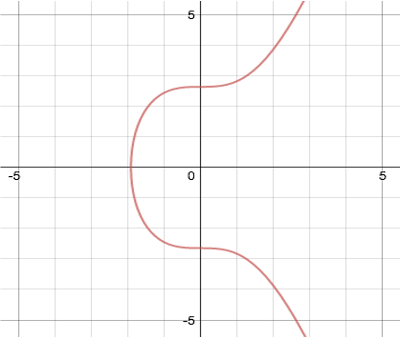
\includegraphics[width=8cm, height=6cm]{charts/1.png}

\begin{flushleft}
Elliptical curves have useful properties. For example, a nonlinear line that intersects two non-tangent points in a curve always passes through the third point on the curve. Another feature is that the non-vertical line tangent to the curve at one point intersects exactly another point on the curve. Using these features, we can define two other operations: adding a dot and doubling the coordinates of a point.\newline

Adding a point with the formula P + Q = R to achieve the x-axis coordinates is the third intersection point R on a line that includes P and Q. This definition is easier to understand as follows:
\end{flushleft}

\centering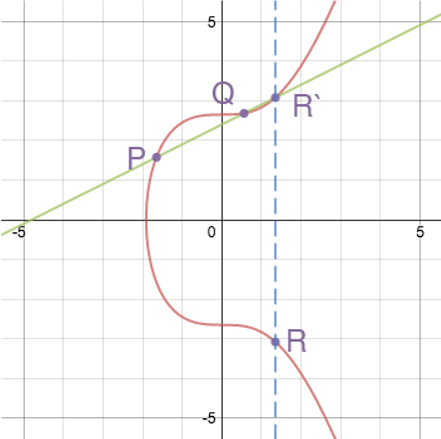
\includegraphics[width=8cm, height=6cm]{charts/2.png}

\begin{flushleft}
Doubling the coordinates of a point with the formula P + P = R and finding the line of tangent to the point whose coordinates are to be doubled and obtaining the coordinates of the x-axis is the intersection point R. Here's an example:

\end{flushleft}

\centering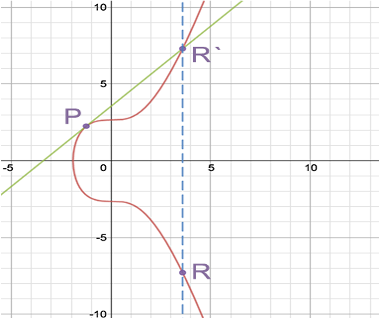
\includegraphics[width=8cm, height=6cm]{charts/3.png}

\begin{flushleft}
These two operations together to multiply the scalar by the formula R = a P and the sum of the point P with it are a. For example, we have:
\begin{equation}
R=7P,\newline
R=P+(P+(P+(P+(P+(P+P)))))
\end{equation}

The scalar multiplication process is usually made easier by combining point addition operations and doubling point coordinates. For example, we have:

\begin{equation}
R=7P,
R=P+6P,
R=P+2(P+2P)
\end{equation}

\subsection{Finite fields}
A finite field, in the context of ECDSA, can be thought of as a predefined range of positive numbers within which every calculation must fall. Any number outside this range “wraps around” so as to fall within the range.

The simplest way to think about this is calculating remainders, as represented by the modulus (mod) operator. For example, 9/7 gives 1 with a remainder of 2:

9 mod 7 = 2

Here our finite field is modulo 7, and all mod operations over this field yield a result falling within a range from 0 to 6.

\subsection{Putting it together}

ECDSA uses elliptic curves in the context of a finite field, which greatly changes their appearance but not their underlying equations or special properties. The same equation plotted above, in a finite field of modulo 67, looks like this:
\end{flushleft}
\centering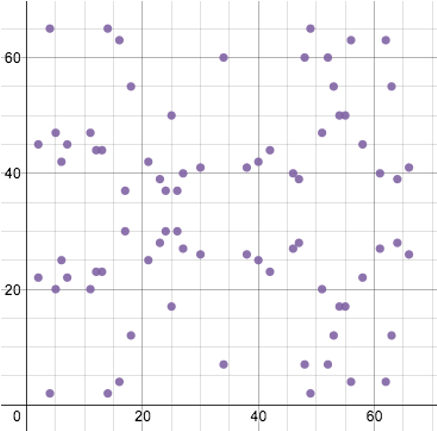
\includegraphics[width=8cm, height=6cm]{charts/4.png}

\begin{flushleft}
It’s now a set of points, in which all the x and y values are integers between 0 and 66. Note that the “curve” still retains its horizontal symmetry.

Point addition and doubling are now slightly different visually. Lines drawn on this graph will wrap around the horizontal and vertical directions, just like in a game of Asteroids, maintaining the same slope. So adding points (2, 22) and (6, 25) looks like this:
\end{flushleft}

\centering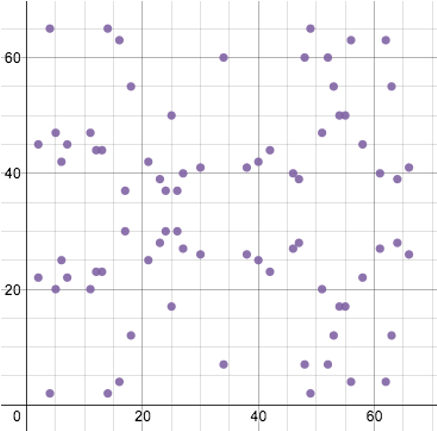
\includegraphics[width=8cm, height=6cm]{charts/4.png}

\begin{flushleft}
The third intersecting point is (47, 39) and its reflection point is (47, 28).

A protocol such as bitcoin selects a set of parameters for the elliptic curve and its finite field representation that is fixed for all users of the protocol. The parameters include the equation used, the prime modulo of the field, and a base point that falls on the curve. The order of the base point, which is not independently selected but is a function of the other parameters, can be thought of graphically as the number of times the point can be added to itself until its slope is infinite, or a vertical line. The base point is selected such that the order is a large prime number.

Bitcoin uses very large numbers for its base point, prime modulo, and order. In fact, all practical applications of ECDSA use enormous values. The security of the algorithm relies on these values being large, and therefore impractical to brute force or reverse engineer.

In the case of bitcoin:

Elliptic curve equation: 
\begin{equation}
y^2 = x^3 + 7
\end{equation}
Prime modulo = 2256 – 232 – 29 – 28 – 27 – 26 – 24 – 1 = FFFFFFFF FFFFFFFF FFFFFFFF FFFFFFFF FFFFFFFF FFFFFFFF FFFFFFFE FFFFFC2F
Who chose these numbers, and why? A great deal of research, and a fair amount of intrigue, surrounds the selection of appropriate parameters. After all, a large, seemingly random number could hide a backdoor method of reconstructing the private key. In brief, this particular realization goes by the name of secp256k1 and is part of a family of elliptic curve solutions over finite fields proposed for use in cryptography.



\subsection{Conclusion}

In this article, we explain the complex mathematical relationship between the public key and the private key. We have also seen how, even in the simplest of examples, the mathematical principles of signatures and verification become so complex. We accept this very complexity when the present parameters are 256-bit numbers. In this paper, we found that the clever use of the simplest mathematical procedures can create the necessary one-way path to maintain information asymmetry that defines bitcoin ownership. We have also regained the strength of this system, which includes completely secure protection of our private keys.
In other words, it is said that bitcoin is supported by mathematics. If you are interested in complex coding issues, we hope this article helps you take the next step in the discussion.\textcite{rykwalder_2014}

\section{Design}
Now, with the algorithms mentioned and the necessary processes in the blockchain, we examine the languages available for this purpose.g


\section{Choosing a programming Language}
If we want to become a blockchain developer, the first step is to choose a programming language that is determined by the type of project you have. In fact, there is no single programming language for blockchain programming, because as you change the way your project works, so does the programming language. For example, a person may choose the Python language to carry out their blockchain project, while another developer may use JavaScript.

So you need to first determine what digital currency can be the basic platform for your project, and you need to determine what you expect from the operation and purpose of that project. To view the best and most popular programming languages in 2020, you can use the articles published on IEEE and tiobe.com.
Accordingly, blockchain programming can be divided into 4 areas of work:
\begin{enumerate}
\item Creating and upgrading a blockchain network
\item Fabric hyperlink project to implement a decentralized general ledger
\item Launch an ICO
\item Build smart contracts and decentralized 
\end{enumerate}
programs (Dapp)
The first challenge is language security, programming. Because blockchain code is public and visible to all users, anyone can check the code and even make changes to it, so a hacker can infiltrate the network by finding security bugs. Steal millions of dollars or digital currency.
The second challenge is resource management. This means that the development of blockchain must be in line with the needs of the network. Because it is not possible to make the necessary predictions from the beginning of the project, it is best for the system to be prepared for questions from around the world or local questions. On the other hand, blockchain design should be the best way to create performance. Therefore, it will be important to use a flexible writing program that can run different instructions in parallel.

In the third challenge, the efficiency and performance of programming languages is assessed.
As mentioned, a blockchain should always display its highest capabilities. Therefore, the use of digital signatures improves the ability to parallelize the blockchain. You don't need anything more than a transaction, a signature, or a key to confirm a digital signature, and with these three confirmations, you can do the tasks in parallel. This feature is evident in all functions of a blockchain

\subsection{C++ Programming Language}
Language, C ++ Programming Program (C ++)
This language was developed by Strostrop more than 30 years ago. In addition to having all the key features of a C-programming language, such as flexibility, security, and efficiency, C ++ has tried to increase the concept of object-orientation. That's why C ++ is known as an object-oriented programming language, but C is a structured programming language.
Many Chinese blockchain developers are currently using the C ++ programming language to design the original ChinaClock core. However, due to the high dependence of C ++ on the type of old variables and commands, its use is not recommended for novice programmers. However, if you are proficient in using this programming language, you will gain a deep understanding of other programming languages.
Language J Java Program Writing
The Java programming language is the king of HTML / Css web pages, and is used to create high-security confidential blockchains because of its immutability, which prevents hacking and sabotage.

\subsection{Go(Language)
}
The Golang programming language, or GO for short, was created by Google in 2007, but over time, with the recognition of its performance in 2012, it was welcomed by the community of programmers. Go is a powerful, multi-purpose programming language that is simple, efficient, and secure. In addition, Go is an interpretive language and is able to work directly with operating systems. This feature has led to the use of this language in various areas of project development based on China.
Atrium SDK has now created a protocol based on the GO programming language, which is used to change a blockchain. The Linux Foundation also uses the Go language to develop high-tech fabric projects.

\subsection{Python Programming Language
}
Python was created by Guido van Rossum with the aim of creating simplicity and readability in the codes and commands of a language program. Many people who have just entered the world of "programming" are very interested in the Python language, because it is easy to learn and the language of "programming" is modern and efficient.
Although the Python language alone cannot create a blockchain-based structure, it must be said that in almost all blockchains, there is one or more general tools with or for Python.
\subsection{JavaScript 
}
JavaScript is the first programming language to be developed to create user interfaces and improve CTML and CSS pages. Today, almost all browsers support JavaScript well.
With the help of intermediaries such as animations, user menus, chat boxes, and interactive maps, Javascript has been able to evolve and improve the behavior of web pages in new and modern browsers. JavaScript is one of the languages of programming that is evolving and improving day by day and is relatively easy for beginners.
The use of JavaScript in blockchain-based projects was first used on the Lisk platform.
The developers of the Lisk project believe that JavaScript can implement a complete ecosystem on the blockchain. Therefore, the Lisk platform has made it possible for programmers to create and implement cloud-based programs in JavaScript.
Selection of auxiliary functions
Python is used to write this project. The reason for this choice is the existence of many libraries and additional auxiliary functions in this language, which speeds up the "writing program" operation. In this section, we will get acquainted with the components that help us.
\subsection{Sha encryption:
}
SHA-256 belongs to the SHA-2 Hash Encryption Functions family, designed by the NSA. Secure Hash Algorithms (SHA) is one of Hash's secure algorithms. Encrypted hash functions are a series of mathematical operations that are applied to digital data; a person can compare the hash calculated (output from the hash algorithm) with the amount of hashish expected of him / her, and can verify the accuracy of a data. Recognize. Data can be converted to hash in a one-way process, but the generated hash cannot be converted to primary data.
 The Sha-256 algorithm is based on the Merkle-Damgard structural method. Accordingly, the initial information is immediately divided into blocks, and after the changes that are made on it, the initial information becomes a 16-word output.
SHA-256 is used in various parts of the Bitcoin network: Extraction uses SHA-256 as a proof-of-work algorithm. SHA-256 is used to create Bitcoin addresses to improve security and privacy.

\subsection{Data conversion with Json:
}
JSON The acronym JavaScript Object Notation means "JavaScript object marking". Of course, don't pay too much attention to its meaning, because translating these phrases usually doesn't give a precise meaning.
Jason often uses a web server to send data to a web page.
Jason himself is self-describing Its codes are very easy due to the name / value structure.

\subsection{Sha encryption:
}
SHA-256 belongs to the SHA-2 Hash Encryption Functions family, designed by the NSA. Secure Hash Algorithms (SHA) is one of Hash's secure algorithms. Encrypted hash functions are a series of mathematical operations that are applied to digital data; a person can compare the hash calculated (output from the hash algorithm) with the amount of hashish expected of him / her, and can verify the accuracy of a data. Recognize. Data can be converted to hashes in a one-way process, but generated hashes cannot be converted to primary data.
 The Sha-256 algorithm is based on the Merkle-Damgard structural method. Accordingly, the initial information is immediately divided into blocks, and after the changes that are made on it, the initial information becomes a 16-word output.
SHA-256 is used in various parts of the Bitcoin network: Extraction uses SHA-256 as a proof-of-work algorithm. SHA-256 is used to create Bitcoin addresses to improve security and privacy.
Data conversion with Json:
JSON The acronym JavaScript Object Notation means "JavaScript object marking". Of course, don't pay too much attention to its meaning, because translating these phrases usually doesn't give a precise meaning.
Jason often uses a web server to send data to a web page.
Jason himself is self-describing, meaning that it's easy to understand its codes because of the name / value structure.

\subsection{Routing with Flask:
}
Flask is a Python-based web framework for creating fast and simple web servers developed by ArminerRunacher. Trying to simplify the design of the small and small frameworks and not giving many defaults to programmers is the reason why this package is called "software software". flask is free and open source and is licensed under the BSD.
Some of the strengths of Philosophy that encourage programmers to use are:
Flask is very easy to learn. If you're a little familiar with the Python language, you'll be able to get rid of it by looking at the code's code.
When working with Flask, you are free to do things as you wish. This means that this framework is quite flexible.
There is a strong community behind the Python language and the Philosophical Framework that you can count on when a problem arises.

\subsection{RSA encryption:
}
In all symmetric encryption algorithms with a symmetric key, the sender and receiver of the message must know the encryption key. When the sender of the message uses a unique, secret key for encryption, and the recipients of the message use the same key to decrypt it, disclosing the password via one of the recipients of the message endangers everyone's security. In such a situation, the sender will have to agree with each recipient individually on a symmetrical secret key so that each receiver has its own key and its disclosure does not interfere with the security of others. In this case, the sender of the message must define and hold the key to the number of recipients. Defining, for example, tens of thousands of symmetrical keys for users and storing and retrieving them safely is a big problem.
In public key algorithms, two completely different keys are used for encryption and decryption: "public key" and "private key".
The public key is used to encrypt information and everyone knows it, because this key is only used to encrypt information, and enemies will not be able to decrypt the data encrypted by others.
A private key is the key with which encrypted data is decrypted. No one, not even trustees and friends, knows this key. Thus, any network-level entity (whether user, machine, or process) needs two independent keys, only one of which is sensitive and secretive and must be carefully maintained. The nature of the encryption algorithm is such that in practice it is not possible to infer a private key by holding a public key.
In the following year, three people named Ryost, Shamir, and Adelman introduced an algorithm for implementing public key encryption with a pair of keys, known as RSA, which has been widely used over the last three decades and over time, optimized hardware and software. It was launched. Although a stronger algorithm called El Gamal was later developed, the RSA method is still at the top of the list of public key algorithms.
Suppose the sender of the pair message has an integer (e, n) as the public key to encrypt their information. On the opposite side, the receiver also uses a pair of numbers (d, n) to decrypt the message. Obviously, the two pairs of numbers (e, n) and (d, n) have a clever relationship with each other, but it is not possible to easily deduce d by having e and n. Assuming that such keys exist, the RSA algorithm Finally, the simplicity is as follows:
A) The message to be encrypted is divided into character K blocks (k bytes).
B) Each block is converted to an integer called Pi according to a completely arbitrary rule.
C) With the pair of numbers (e, n) for each Pi block, new numbers are obtained according to the following relation:
Ci = (Pi) e mod n
D) Ci codes are sent instead of the original Pi codes.
The method of decrypting the data is exactly the same as the encryption method, ie by having a pair of numbers (d, n), the encrypted blocks are decoded as follows. Should:
Pi = (Ci) d mod n
The whole algorithm ends here.
In RSA, the pair of numbers (e, n) with which the text is encrypted, the so-called public key, and the pair of numbers (d, n) through which the text is encrypted, the private key. Called. The basic point in RSA is that in order to ensure the inversion of the cryptographic method, the numbers must be true for the relation (x) e.d mod n = x, so care must be taken in the selection of numbers.
Another basic principle that must be followed in RSA encryption is that the Pi codes that we assign to each block must be in the 0 <= Pi <n condition. Therefore, if the blocks are modeled as k-bit strings, the 2K <n condition must be met. The reason for this is that it is easy to write the statement Pi mod n = Pi, otherwise, in general, this statement is not correct, and in this case, the correct decryption of the data will not be guaranteed.
The e and d selection methods proposed by RSA inventors are:
A) Two arbitrary (but large) numbers p and q are selected.
B) The numbers n and z are calculated according to the following two relations:
n = p * q
z = (p-1) * (q-1)
C) The number d is selected so that it is equal to the first z, meaning that no common factor is found on which both are divisible.
D) Based on d, the number e is selected so that the following relation is established: (In other words, the multiplicative multiplication of d in the measure of z is calculated and called e)
(e * d) mod z = 1
What is clear is that in practical applications, the numbers p and q are selected at least one hundred digits (one hundred digits in base ten), meaning that these two numbers are at least.. In this case, the correct number corresponding to the Pi blocks, which according to the above condition must be less than n, must not be more than 2 characters,
So each text block must have a maximum of 2 bits or 8 bits.
Here, it is necessary to note that in order to calculate Ae mod n, it is not necessary to multiply A by the number of e loads and then find its remainder on n, because using some mathematical properties, the result of the calculations never exceeds n.
Now suppose an intruder wants to get public by having the general key (e, n).. In this case, he must first decompose n into its first two factors, p and q, so that he can calculate z and Then he got d. There is no way to break down numbers into the first factor except by searching and testing, and given that n is at least two hundred digits, it will take thousands of years, even with the help of a computer.
Although research on the problem of decomposing large numbers into its factors is still ongoing, an efficient algorithm that can decompose large numbers at any time in fixed time or in small quantities has not yet been found. The year since the introduction of the RSA has not diminished its value, but only the keys have been enlarged to do so.
Since the first numbers have no known order, so choosing the first very large numbers p and q is one of the big challenges of RSA because to prove that a number like p is the first, the range of lesser or equal numbers p should be examined and p pivability studied.
The larger the p, the larger the search range .p. For example, the search range for numbers becomes 512 bit., Which makes it virtually impossible to search for such space. So the only solution is to use a series of mathematical theorems that help us narrow down the search range and reduce the guesswork.
\subsection{Binascii}
The binascii module includes a number of methods for converting between binary and different encrypted ASCII binary displays. Typically, you do not use these functions directly, but use packing modules.
\section{Conclusion:
}
According to the concepts, assumptions and study of all encryption algorithms required is the language that designed the existing algorithms in the simplest and fastest possible way. Python is a programming language that, with its rich and extensive libraries, speeds up project design faster and more powerfully.
\end{flushleft}


\chapter{Implementation}
\begin{flushleft}

\section{not here for now}
The code is available commented and explained in git and persian article.\linebreak

\href{https://github.com/MohsenDehbag/thesis-about-blockchain}{Click on this line to view at the code on github.}
\end{flushleft}


\chapter{Conclusion}
\section{Conclusions and the Future of Blockchain}
Blockchain is a new technology that must overcome a number of problems before its full advantages
can be exploited, but so was the Internet before October 1990, when Sir Tim Berners-Lee introduced
three fundamental technologies that formed the foundation of the World Wide Web (WWW) and are
utilized until today. By the end of 1990, the first web page was posted on the internet, which people
could visit and view information on, mostly transmitted through modems and regular telephone
lines. However, such information consisted of text only characters, as sounds, images and videos
were outside the communication capabilities of that time. Google, Amazon, Facebook, or YouTube
were unimaginable at that time, when even sending an email, before the Mosaic web browser was
introduced, was considered a technological achievement. Nobody should be surprised, therefore, with
blockchain’s current limitations, as it is at around the same stage as the Internet was in the mid-1990s.
In this paper we discussed the core advantages of blockchain and pointed out that its full potential
would be unleashed in the not too distant future [40], with new giant firms, the equivalent of Google,
Amazon, and Facebook, emerging to exploit the advantages of blockchain technologies. In this
conclusion, we would like to reiterate the value of blockchain and its disruptive nature while also
deliberating about its future achievements. A recent Deloitte Global Blockchain Survey  concluded
that 2019 was a turning point for blockchain when a radical shift happened in the attitudes of business
leaders who recognized that blockchain is for real and that it can serve as a pragmatic solution to
business problems across industries and use cases. That is, these leaders recognized a shift from
“blockchain tourism” and exploration towards the building of practical business applications, as
blockchain has finally entered the mainstream of business applications. Blockchain guarantees trust,
assures immutability, transparency, and supports disintermediation in addition to providing extra
security for transactions executed over the Internet. These are considerable advantages that cannot
be ignored, while its disadvantage of the cost of implementation can be depreciated and reduced in
a short amount of time, as more experience with applications is gained and blockchain becomes a
core technology. Most importantly, however, as usage increases the motivation for improvements will
increase, too, as has been the case with the Internet that witnessed substantial advancements over
a short period of time. Such advancements will provide solutions to blockchain’s inability to scale,
significantly reducing usage costs.
Blockchain’s ability towards security and immutability can also be used for storing the highly
sensitive, personal data needed to determine patterns in sensitive cases such as those involving the
healthcare sector. Furthermore, blockchain can contribute to breaking the black box of AI by tracing
how algorithms work and how their input affects the output of machine learning, while AI can increase
the efficiency of blockchain far better than humans, or standard computing. Finally, Bitcoin, viewed as
blockchain’s first innovative success , can contribute to applying the technology to additional areas,
increasing the popularity of both Bitcoin and AI, as well as their various applications. Blockchain and
AI are new technologies and much will depend on future, yet unknown, technological advancements.
However, there is considerable potential that can raise their separate, as well as their combined,
usefulness to new, high levels of value and applicability. This has been the case with the Internet, as
well as, all new technologies whose future value has been underestimated greatly at the outset.


\end{document}
